%FILL IN THE RIGHT INFO.
%\lecture{**LECTURE-NUMBER**}{**DATE**}
\unchapter{Lecture 8}
\lecture{8}{September 29}
\setcounter{section}{0}
\setcounter{theorem}{0}

% **** YOUR NOTES GO HERE:

We begin with a small remark, inspired by a previous homework set

\begin{remark}
Let $\gamma_1, \gamma_2$ be parameterized piecewise smooth curves, with the same initial points and end points, and such that they do not cross except at endpoints (they enclose a region $\Omega$). If $f$ holomorphic on $\overline{\Omega}$ then $\int_{\gamma_1}f(z) \dif z = \int_{\gamma_2} f(z) \dif z$. This follows easily by Cauchy's Theorem, since $0 = \int_{\partial \Omega} = \int_{\gamma_1} = \int_{\gamma_2}$.

\begin{center}
\begin{tikzpicture}[very thick,decoration={
    markings,
    mark=at position 0.5 with {\arrow{>}}}
    ]

\draw[fill] (-3,-1) circle [radius=2pt];
\draw[fill] (3,1) circle [radius=2pt];

\draw plot [smooth, tension=2] coordinates { (-3,-1) (-2,2) (0,1.5) (1,2) (3,1)};
\draw plot [smooth, tension=2] coordinates { (-3,-1) (-1,-1) (0,1) (3,0) (3,1)};


\draw (-0.1,1.5-0.1) -- (0,1.5) -- (0-0.1,1.5+0.1);
\draw (0-0.9*0.14,1+0.4*0.14) -- (0,1) -- (0-0.4*0.14,1-0.9*0.14);

\draw (0,1.5)[above] node {$\gamma_1$};
\draw (0,1)[below] node {$\gamma_2$};
\draw (-1.5,0) node {$\om$};

\end{tikzpicture}
\end{center}


This does not hold if $f$ is not holomorphic on $\overline{\Omega}$. Consider $f(z)= \frac{1}{z}$. Then we have calculated (in an excluded example) that with $\gamma_1$ the upper half unit circle and $\gamma_2$ the lower half unit circle that $\int_{\partial D_1(0)} f(z) \dif z = \int_{\gamma_1} f(z) \dif z + \int_{\gamma_2} f(z) \dif z = 2\pi i \neq 0$.
\end{remark}




\begin{center}
\begin{tikzpicture}[very thick,decoration={
    markings,
    mark=at position 0.5 with {\arrow{>}}}
    ]
    \draw[postaction={decorate}][xscale=1][rotate = 90] (0,0) circle [radius=1];
    \draw[postaction={decorate}][xscale=-1][rotate = -90] (0,0) circle [radius=1];
    
    \draw[fill] (-1,0) circle [radius=2pt];
    \draw[fill] (1,0) circle [radius=2pt];
    
    \draw (0,1)[below] node {$\gamma_1$};
    \draw (0,-1)[above] node {$\gamma_2$};
    \draw (-1,0)[right] node {$\om$};
    \draw[thick] (-0.1,0.1) -- (0.1,-0.1);
    \draw[thick] (0.1,0.1) -- (-0.1,-0.1);
    
\end{tikzpicture}
\end{center}





We now look at a comparatively non-trivial theorem. Montel's Theorem give us a sufficient an necessary condition for a family of holomorphic functions on a domain to converge uniformly on compact sets to some limit.


\section{Montel's Theorem}

\isubsection{THM: Montel's Theorem}
\begin{theorem}[Montel's Theorem]
$f_n: \om \to \C$ holomorphic functions, $n \in \mathbb{N}$. Suppose that they are uniformly bounded on compact subsets of $\om$ (ie $\forall K \ssubset \om $ compact $ \exists C > 0 $ s.t. $ \sup_{z \in K} \abs{f_n(z)} \leq C \, \forall n)$. Then $\exists $ subsequence $n_j \to \infty, \, \exists \foc  $ holomorphic s.t. $f_{n_j} \tou f$ on compact subsets  of $\om$ and $f_{n_j}^{(k)} \tou f^{(k)}$ on compact subsets of $\om , \, \forall k \geq 0$.
\end{theorem}


\begin{definition}[Normal Family]
A set of functions is called a \textbf{normal family} if $\exists $ subsequence $n_j \to \infty$ and $ \exists \foc  $ holomorphic s.t. $f_{n_j} \xrightarrow[]{u} f$ on compact subsets  of $\om$ and $f_{n_j}^{(k)} \xrightarrow[]{u} f^{(k)}$ on compact subsets of $\om , \, \forall k \geq 0$.\\

Note that the case where $k=0$ is simply the first sentence, and that if the $k=0$ case holds the $k>0$ case is implied. Thus, it is sufficient to ignore the $k>0$ case when writing the definition.
\end{definition}


\begin{remark}
Montel's Theorem states that for a set of functions, uniformly bounded on compact subsets implies normal.

If $f_n \tou f$ holomorphic on compact subsets then $f_n$ is uniformly bounded on compact subsets. Without the subsequence part, being a normal family is essentially equivalent to being uniformly bounded on compact sets.
\end{remark}


\begin{remark}
$\{ f_n \}$ uniformly bounded on compact subsets of $\om$ $\iff$ $\{ f_n \}$ locally uniformly bounded (ie $\forall \, z_0 \in \om, \, \exists \, r,C > 0 $ s.t. $ D_r(z_0) \ssubset \om$ and $\sup_{z \in D_r(z_0)} \abs{f_n(z)} \leq C$).

The right direction is simple, as each disk is covered by a compact set that is still in $\om$. To see the left direction, cover a compact set with disks. By compactness, we can reduce the cover to finitely many disks. Take the maximum of the finitely many constants, and you are done.
\end{remark}

\begin{remark}
Content of Montel is that it strengthens Ascoli-Arzelà by removing the assumption of equi-continuity. It also strengthens it by proving the statement for all the derivatives.

Conversely, Ascoli-Arzelà doesn't need holomorphic (merely continuous), while Montel does.
\end{remark}

\begin{proof}[Montel's Theorem] This is a consequence of the Cauchy integral formula and the Cauchy estimates. Let us first prove that $\{ f_n \} $ is equicontinuous on compact subsets of $\om$.

We must show that $\forall K \ssubset \om$ compact $\forall \epsilon >0 \, \exists \delta$ s.t. if $ x,y \in K, \abs{x-y} < \delta $ then $ \abs{f_n(x) - f_n(y) } < \epsilon, \, \forall n$.

Since K compact and $\om$ closed, $dist(K, \partial \om) > 3r >0 $ for some $r$. Let $z,w \in K$ s.t. $\abs{z-w} < r$. Take a disk $z \in D = D_{2r}(w) \subset \om$ of radius $2r$ around $w$.


\begin{center}
\begin{tikzpicture}
    \draw (0,0) circle (3);
    
    \draw[dotted][scale =1]plot [smooth] coordinates { (4,6) (5,5) (6,2.5) (8,0) (7,-3) (6.5,-4)};
    
    \draw[dotted][scale =1] plot [smooth] coordinates { (-1,4) (1,3) (2,1) (2.1,0) (2,-3) (1, -3.5) };
    
    \draw (0,0)[below left] node {$w$};
    \draw[fill] (0,0) circle [radius=2pt];
    
    \draw (70:1.2)[above left] node {$z$};
    \draw[fill] (70:1.2) circle [radius=2pt];
    
    \draw (-30:3)[right] node {$\zeta$};
    \draw[fill] (-30:3) circle [radius=2pt];
    
    \draw (0,0) -- (70:1.2) -- (-30:3) -- (0,0);
    
    \draw (70:0.6) [left] node {$r>$};
    \draw (-30:1.5) [below left] node {$2r$};
    
    \draw (270-20:2.5) node {$D$};
    \draw (120-10-10:4.3) node {$K$};
    \draw (30:7) node {$\om$};
    
    
    
    
    \draw[<->] (2,1) -- (6,2.5);
    \draw (2/2+6/2,1/2+2.5/2) [below right] node {$3r$};
    
    
\end{tikzpicture}    
\end{center}



Apply the Cauchy integral formula to $w$ and $z$ and subtract:

\begin{align*}
    f_n(z) - f_n(w) = \frac{1}{2 \pi i} \int_{\partial D} f_n(\zeta) \left( \frac{1}{\zeta - z} - \frac{1}{\zeta - w}\right) \dif \zeta  \\
\end{align*}

By assumption then since $D\subset K' \subset \om$ for some $K'$, $f_n$ is uniformly bounded independent of n. Then:

\begin{align*}
    \abs{w-\zeta} &= 2r\\
    \abs{w-z} &< r\\
    4r \geq \abs{\zeta - z} &= \abs{\zeta - w + w -z}\\
    &\geq  \underbrace{\abs{\zeta - w}}_{=2r} - \underbrace{\abs{w-z}}_{<r} > r\\
\end{align*}

Thus:

\begin{align*}
    \abs{\frac{1}{\zeta - z} \frac{1}{\zeta - w}} &= \frac{\abs{z-w}}{\abs{\zeta-z} \cdot \abs{\zeta-w}}\\
    &\leq \frac{\abs{z-w}}{2r\cdot r} = \frac{\abs{z-w}}{2r^2}
\end{align*}

Taking the modulus of the Cauchy integral formula:

\begin{align*}
    \abs{f_n(z) - f_n(w)} &\leq \frac{1}{2 \pi i} \int_{\partial D} \underbrace{\abs{f_n(\zeta) }}_{u.bd. <C} \cdot \frac{\abs{z-w}}{2r^2} \dif \zeta\\
    \text{(for some constant $\Tilde{C}$) }& \leq \Tilde{C} \abs{z-w} \forall n
\end{align*}

This shows that the family $\{ f_n \} $ is equicontinuous and uniformly bounded on compact subsets of $\om$. Thus we can apply Ascoli-Arzelà. Thus, $\forall K \ssubset \om$ compact, $\exists n_j \to \infty$ subsequence, $\exists f \in C^0 (K) $ s.t. $f_{n_j} \tou f$ on K. From last time, $f$ is holomorphic on $\interior{K}$.

We must now show that $f_n \tou f$ on all compact subsets (now we have proved that for any compact set, there is some subsequence that converges on that compact set) and that the derivatives converge.

We apply a diagonal argument. We can find an exhaustion $\{ K_i \}$ of $\om$ by compact subsets:

\begin{align*}
    K_1 \subset K_2 \subset \cdots \subset K_j \subset K_{j+1} \subset \cdots \om\\
\end{align*}
Such that $K_j \subset \interior{K}_{j+1} \, \forall j$ and that $\bigcup_{j=1}^\infty K_j = \om$



\begin{center}
    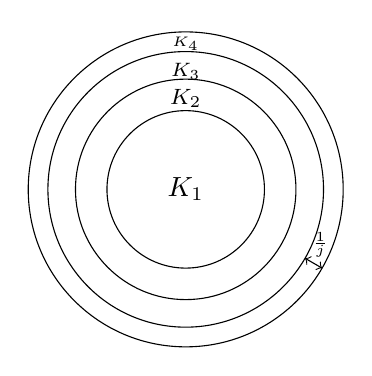
\begin{tikzpicture}
    
    \draw (0,0) circle (2);
    \draw (0,0) circle (1);
    \draw (0,0) circle (1.4);
    \draw (0,0) circle (1.75);
    
    \draw node at (0,0) {$K_1$};
    \draw node at (0,1.15) {\footnotesize $K_2$};
    \draw node at (0,1.5) {\scriptsize $K_3$};
    \draw node at (0,1.85) {\tiny $K_4$};
    \draw[<->] (-30:1.75) -- (-30:2);
    \draw node at (-22.5:1.851) {\tiny $\frac{1}{j}$};
    \draw [below right] node at (-45:2) {$\om$};
    
    
    \end{tikzpicture}
\end{center}




%REVISE

e.g. $K_j = \set{ z \in \C \mid dist(z,\partial \om) \geq \frac{1}{j} } \cap \overline{D_j(0)}$ (the disk of radius $j$ around the origin is to ensure boundedness). Now apply the first part of the proof to $K_1$ to get $\{ f_{n,1} \} $ a subsequence of $\{f_n\}$ s.t. $ f_{n,1}  \xrightarrow[]{\interior{C}(K_1)} f$, $f \in \interior{C} (K_1)$, $f$ holomorphic on $\interior{K}_{1}$. Now apply the first part of the proof to $K_2$ and the family $\{ f_{n,1} \}$. This yields a sub-subsequence $f_{n,2} \xrightarrow[]{\interior{C}(K_1} \Tilde{f}$, $\Tilde{f} \in \interior{C}(K_2)$ holomorphic on $\interior{K}_{2}$. The uniform limit is unique, thus $f = \Tilde{f}$ on $K_1$ by uniform convergence.

Repeat this procedure to $\{ f_{n,2} \}$ on $K_3$ to get $\{ f_{n,3} \}$ etc. Finally take the sequence $\{ f_{n,n} \}_{n=0}^\infty$. By construction, $f_{n,n} \tou f$ on all compact subsets of $\om$.


This proves the first part of Montel's Theorem. The statement about the derivatives remains to be proved. For convenience, relabel so that $f_n \tou f$ on all compact subsets of $\om$. $\forall k \geq 0$, given any point $z_0 \in \om$, take $D = D_r(z) \ssubset \om$ for some $ r> 0$. Apply the Cauchy estimates to the function $f_n^{(k)} - f^{(k)}$:

\begin{align*}
    \forall z \in D_{\frac{r}{2}} (z_0) 
    \: z\abs{f_n^{(k)}(z) - f^{(k)} (z) } \leq \frac{k!}{r^k} \sup_{\partial D} \abs{f_n - f} \xrightarrow[]{f_n \xrightarrow[]{u} f} 0\\
\end{align*}

Where $\sup_{\partial D} \abs{f_n - f} \to 0$ since $f_n \tou f$ on $\overline{D}$. Hence $f_n^{(k)} \to f^{(k)}$ locally uniformly $\implies$ $f_n^{(k)} \to f^{(k)}$ uniformly on all compact subsets of $\om$. This is what we wanted to prove, hence we are done.

\end{proof}

\subsection{Some Examples}

\begin{example}
For $C^\infty$ real functions this fails. Consider $f_n(x) = \sin(nx)$ on $[0,1] \subset \R$.

$f_n$ are uniformly bounded smooth functions, but they are not equicontinuous, and in fact have no convergent subsequence on any compact subset of $[0,1]$


\end{example}


\begin{example}

Consider $\oic$ open, $\om ' \subset \C$ open and bounded. Note that $\F = \set{ f: \om \to \om ' \mid f \, holomorphic  }$. Then $\F$ is normal. This is because $\forall f \in \F, \, \sup_{\om} \abs{f} \leq diam(\om ')$, which is finite since $\om ' $ is bounded.

\end{example}


\begin{note}
The concept of normal families extends very easily to uncountable sets in the obvious way (still looking at countable sequences).
\end{note}

\begin{remark}
Part 3 of the proof shows that if $\F$ is a normal family of holomorphic function $\om \to \C$, then $\forall k\geq 0, \, \F^{(k)} = \set{f^{(k)} \mid f \in \F}$ is also normal. This will be used later in the course.
\end{remark}

We now move backwards in the textbook, back to our original location of chapter 3.


\section{Isolated Singularities, Poles}

Recall from last time: $\oic $ open connected, $\foc$ holomorphic, $f \nequiv 0$. Then given $z_0 \in \om, \exists D $ disk containing $z_0$. $\exists N \geq 0$ and holomorphic s.t. $g(w) \neq 0 \, \forall w \in D$ s.t. $f(z_0) = (z-z_0)^N \cdot g(z) $ on D.

Recall that we defined the unique $N$ in the previous section to be the order of vanishing, and that when $N=1$ we call $z_0$ a simple zero.


Say now that instead of a zero we have a singularity, $z_0 \in \om , \, f: \om \setminus \{ z_0 \} \to \C$ holomorphic on $\om \setminus \{ z_0 \}$.


\begin{center}
\begin{tikzpicture}
    \draw[shift={(-2.5,-2.5)},rotate=0][dotted][scale =2.5] plot [smooth cycle] coordinates {(0,0) (1,0.1) (2,0.3) (2,0.7) (1.5,1.5) (0.8,1.5) (0.3,1.2) (-0.2,0.6) };
    \draw (-2.25,-2.25) node {$\Omega$};
    
    \draw[thick] (-0.1,0.1) -- (0.1,-0.1);
    \draw[thick] (0.1,0.1) -- (-0.1,-0.1);
    \draw [below left] node at (0,0) {$z_0$};
    \draw[dotted] (0,0) circle (1);
    \draw [below right] node at (-30:1-0.05) {$D$};
    
\end{tikzpicture}    
\end{center}



\begin{definition}[Poles]
We say that $f$ has a \textbf{pole} at $z_0$ if $\exists \, D = D_r(z_0) \subset \om$ for some $r>0$ s.t. $f(z) \neq 0 \, \forall z \in D \setminus \{ z_0 \}$ and the function:

\begin{align*}
    \Tilde{f}(z) \vcentcolon = \begin{cases} \frac{1}{f(z)} & z \in D \setminus \{ z_0 \} \\ 0 & z = z_0  \end{cases}
\end{align*}

is holomorphic on $D$.

\end{definition}

To have a pole means to have a holomorphic function that is not defined at $z_0$  but is holomorphic outside, and must be non-zero on some punctured disk around $z_0$.



\begin{lemma}
Suppose that $f$ has a pole at $z_0$. Then $\exists D \ni z_0$ disk, $\exists g: D \to \C $ holomorphic, $g(z) \neq 0 \, \forall z \in D$ and $\exists ! N \geq 1$ such that $\forall z\in D \setminus \{ z_0 \}$:

\begin{align*}
f(z) = \frac{g(z)}{(z-z_0)^N}    
\end{align*}

\end{lemma}

\begin{example}
$\frac{1}{z}$ at $z_0 = 0$ is the prototype of a pole.
\end{example}

\begin{example}
$\frac{1}{z^n}$, $n \geq 1$ at $z_0 = 0$ is also a pole.
\end{example}

\begin{proof}
Since $f$ has a pole, let $\tilde{f}$ be the function described above. $\tilde{f}: D \to \C$ holomorphic. By assumption $f$ is never 0. Thus by construction, $\tilde{f}$ is non-zero except at the isolated zero $z_0$. By the proposition from last time we can write:

\begin{align*}
    \tilde{f} (z) = (z-z_0)^N \cdot h(z) 
\end{align*}

on some possibly smaller disk at $z_0, \, N \geq 1$ and $h:D \to \C$ holomorphic and non-zero. Now we let:

\begin{align*}
    g(z) = \frac{1}{h(z)}
\end{align*}

and we are done.

\end{proof}

\begin{definition}[Order of Pole]
We call the unique $N$ in the previous lemma the \textbf{order of the pole}. This is the analog to the order of the zero. When $N=1$ we call it a simple pole.
\end{definition}


\begin{lemma}[Laurent Series for Poles]
Suppose that $f$ has a pole of order $N$ at $z_0 \in \om$ ($f$ is implicitly holomorphic on the punctured disk). Then $\exists D \ni z_0$ disk such that for $z\in \DP$:

\begin{align*}
    f(z) = \frac{a_{-N}}{(z-z_0)^N} + \frac{a_{-N+1}}{(z-z_0)^{N-1}} + \cdots + \frac{a_{-2}}{(z-z_0)^2} + \frac{a_{-1}}{z-z_0} + G(z)
\end{align*}

with $a_j \in \C, \, G(z) $ holomorphic on $D$.

Thus we can effectively write on this punctured disk:

\begin{align*}
    f(z) = \sum_{n=-N}^\infty a_n (z-z_0)^n 
\end{align*}

This is the Laurent series of $f$ centered at $z_0$ (a pole).


\end{lemma}

\begin{proof}
Take previous lemma. Then on $\DP$:

\begin{align*}
    f(z) = \frac{g(z)}{(z-z_0)^N} 
\end{align*}

Expand $g$ in power series on D:


\begin{align*}
g(z) = \sum_{n=0}^\infty A_n (z-z_0)^n
\end{align*}

and plug it in:

\begin{align*}
    f(z) &= \frac{1}{(z-z_0)^N} \cdot (A_0 + A_1(z-z_0) + A_2 (z-z_0)^2 + \cdots)\\
    \text{(letting $a_i = A_{i+N}$) } &= \sum_{n=-N}^\infty a_n (z-z_0)^n
\end{align*}
And we are done.
\end{proof}

\begin{definition}[Principal Part and Residue]

When $f$ has a pole at $z_0$ we can write:

\begin{align*}
    f(z) = \sum_{n=-N}^{-1} a_n (z-z_0)^n + \sum_{n=0}^{\infty} a_n (z-z_0)^n
\end{align*}
The first sum is called the \textbf{principal part of $f$ at $z_0$}. $a_{-1} = \vcentcolon Res_{z_0} (f)$ is called the \textbf{residue of $f$ at $z_0$}. Note that $\abs{N} < \infty$.
\end{definition}

\begin{example}
The function
\begin{align*}
f(z) = \frac{1}{z+5}
\end{align*}
has a pole at $z_0 = -5$. The order of the pole is 1. This is the Laurent Series of $f$ at $z_0$, and thus $Rez_{-5}(f) = 1 $.
\end{example}



\begin{example}
The function
\begin{align*}
f(z) = \frac{1}{(z+5)^2}
\end{align*}
has a pole at $z_0 = -5$. The order of the pole is 2. This is the Laurent Series of $f$ at $z_0$, and thus $Rez_{-5}(f) = 0 $.
\end{example}



\begin{example}
The function
\begin{align*}
f(z) = \frac{1}{z^2+1} = \frac{1}{(z-i)(z+i)}
\end{align*}
has two poles: $z = \pm i$. By plugging in $z= \pm i$ and ignoring the division by zero we get that:

\begin{align*}
    Res_i(f) &= \frac{1}{2i}\\
    Res_{-i}(f) &= \frac{-1}{2i}\\
\end{align*}

\end{example}









